\def\year{2017}\relax
%File: formatting-instruction.tex
\documentclass[letterpaper]{article} %DO NOT CHANGE THIS
\usepackage{aaai18}  %Required
\usepackage{times}  %Required
\usepackage{helvet}  %Required
\usepackage{courier}  %Required
\usepackage{url}  %Required
\usepackage{graphicx}  %Required
\frenchspacing  %Required
\setlength{\pdfpagewidth}{8.5in}  %Required
\setlength{\pdfpageheight}{11in}  %Required
%PDF Info Is Required:
  \pdfinfo{}
\setcounter{secnumdepth}{0}

\usepackage{amsmath}
\usepackage{amssymb}
\usepackage{amsthm}
\usepackage{multirow}
\usepackage{tikz}
\usetikzlibrary{arrows,automata}
\usepackage{comment}

\usepackage{graphicx}
\usepackage{caption}
\usepackage{subcaption}
\usepackage{listings}

\lstset{
  basicstyle=\ttfamily,
  mathescape
}


\usepackage{multicol}
\usepackage{arydshln}
\usetikzlibrary{calc,backgrounds,positioning,fit}


\newcommand{\tup}[1]{{\langle #1 \rangle}}

\newcommand{\pre}{\mathsf{pre}}     % precondition
\newcommand{\del}{\mathsf{del}}     % effect
\newcommand{\add}{\mathsf{add}}     % effect
\newcommand{\eff}{\mathsf{eff}}     % effect
\newcommand{\cond}{\mathsf{cond}}   % conditional effect
\newcommand{\true}{\mathsf{true}}   % true
\newcommand{\false}{\mathsf{false}} % false
\newcommand{\PE}{\mathrm{PE}}     % precondition
\newcommand{\strips}{\textsc{Strips}}     % precondition


\newtheorem{theorem}{Theorem}
\newtheorem{lemma}[theorem]{Lemma}
\newtheorem{definition}[theorem]{Definition}


\begin{document}

\title{Model Recognition as Planning}

% Commented for blind submission
\author{Diego Aineto\and Sergio Jim\'enez\and Eva Onaindia \and Miquel Ram\'irez\\
{\small Departamento de Sistemas Inform\'aticos y Computaci\'on}\\
{\small Universitat Polit\`ecnica de Val\`encia.}\\
{\small Camino de Vera s/n. 46022 Valencia, Spain}\\
{\small \{dieaigar,serjice,onaindia\}@dsic.upv.es}}



\maketitle
\begin{abstract} 
Given the partial observation of a plan execution and a set of possible planning models (that share the same state variables but define different action models), {\em model recognition} is the task of identifying which model in the set produced the given observation. The paper formalizes the {\em model recognition} task and proposes a novel method to assess the probability of a \strips\ model to produce a given partially observed plan execution. This method, that we called {\em model recognition as planning}, is robust to missing data (missing intermediate states and actions) in the observed plan execution  besides, it is computable with an off-the-shelf classical planner. The effectiveness of {\em model recognition as planning} is shown in a set of \strips\ models encoding different kinds of {\em finite state machines}. We show that {\em model recognition as planning} succeeds to identify the executed automata despite internal machine states or actual applied transitions, are unobserved.
\end{abstract}

\section{Introduction}
\label{sec:introduction}
{\em Plan recognition} is the task of predicting the future actions of an agent provided observations of its current behavior. Plan recognition is considered {\em automated planning} in reverse; while automated planning aims to compute a sequence of actions that accounts for a given goals, plan recognition aims to compute the goals that account for an observed sequence of actions~\cite{geffner:book:2013}.

Diverse approaches has been proposed for plan recognition such as {\em rule-based systems}, {\em parsing}, {\em graph-covering}, {\em Bayesian nets}, etc~\cite{carberry2001techniques,sukthankar2014plan}. {\em Plan recognition as planning} is the model-based approach for plan recognition~\cite{ramirez2012plan,ramirez2009plan}. This approach assumes that the action model of the observed agent is known and leverages it to compute the most likely goal of the agent, according to the observed plan execution.

This paper introduces the {\em model recognition} task where the target of the recognition process is not a goal but a {\em planning model}. Given a partial observation of a plan execution and a set of possible planning models (that share the same state variables but define different action models), {\em model recognition} is the task of identifying which model in the set has the highest probability of producing the given observation.

\begin{figure}
  \begin{scriptsize}
  \begin{center}
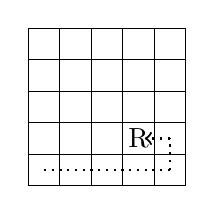
\begin{tikzpicture}[scale=.4]
          \begin{scope}
            \draw (0, 0) grid (5, 5);
            \node[anchor=center] at (3.5, 1.5) {R};
            \node[anchor=center] at (0.5, 0.5) {};
            \draw[thick,style=dotted] (0.5,0.5) -- (4.5,0.5);
            \draw[thick,style=dotted] (4.5,0.5) -- (4.5,1.5);
            \draw[thick,style=dotted,->] (4.5,1.5) -- (3.7,1.5);                        
          \end{scope}
        \end{tikzpicture}
  \end{center}
  \end{scriptsize}  
 \caption{\small Observation of the execution of a robot navigation plan in a $5\times 5$ grid.}
\label{fig:grid-example}
\end{figure}

To better illustrate {\em model recognition}, imagine a robot in a $n\times n$ grid whose navigation is determined by the \strips\ model of Figure~\ref{fig:model-example}. According to this model the robot can increment its {\em x-coordinate} when it is at an {\em even} row while, at {\em odd rows}, can decrement the {\em x-coordinate}. Apart from this particular navigation model, different models can be defined within the same state variables (e.g. altering the way {\small\tt (state-q0)} and {\small\tt (state-q1)} are required and updated) and these models can determine different kinds of robot navigation. Given an observation of a plan execution, like the one illustrated at Figure~\ref{fig:grid-example}, {\em model recognition} aims here to identify which navigation model produced that observation, despite key information is unobserved (e.g. the value of {\small\tt (state-q0)} and {\small\tt (state-q1)} or the particular applied actions). 

{\em Model recognition} is of interest because once the planning model is recognized, then the model-based machinery for automated planning becomes applicable~\cite{ghallab2004automated}. In addition, it enables identifying different kinds of automatae by observing their execution. It is well-known that diverse automatae representations, like {\em finite state controllers}, {\em push-down automata}, {\em {\sc GOLOG} programs} or {\em reactive policies}, can be encoded as classical planning models~\cite{baier2007exploiting,Geffner:FSM:AAAI10,segovia2017generating,ivankovic2015optimal}.

The paper introduces also {\em model recognition as planning}; a novel method to assess the probability of a given \strips\ model to produce an observed plan execution. The method is robust to missing data in the intermediate states and actions of the observed plan execution besides, it is computable with an off-the-shelf classical planner. The paper evaluates the effectiveness of {\em model recognition as planning} with a set of \strips\ models that represent different {\em finite state machines}. All of these {\em automatae} are defined within the same {\em alphabet} and same {\em machine states} but different {\em transition functions}. We show that {\em model recognition as planning} succeeds to identify the executed {\em automata} despite internal machine states or actual applied transitions are unobserved.


\begin{figure}
  \begin{tiny}
  \begin{verbatim}
  (:action inc-x
    :parameters (?v1 ?v2)
    :precondition (and (x-coord ?v1) (next ?v1 ?v2) (state-q0))
    :effect (and (not (x-coord ?v1)) (x-coord ?v2)))

  (:action dec-x
    :parameters (?v1 ?v2)
    :precondition (and (x-coord ?v1) (next ?v2 ?v1) (state-q1))
    :effect (and (not (x-coord ?v1)) (x-coord ?v2)))

  (:action inc-y-even
    :parameters (?y1 ?y2)
    :precondition (and (y-coord ?y1) (next ?y1 ?y2) (state-q0))
    :effect (and (not (y-coord ?y1)) (y-coord ?y2)
                 (not (state-q0)) (state-q1))

  (:action inc-y-odd
    :parameters (?y1 ?y2)
    :precondition (and (y-coord ?y1) (next ?y1 ?y2) (state-q1)))
    :effect (and (not (y-coord ?y1)) (y-coord ?y2)
                 (not (state-q1)) (state-q0)))

  (:action dec-y-even
    :parameters (?y1 ?y2)
    :precondition (and (y-coord ?y1) (next ?y2 ?y1) (state-q0))
    :effect (and (not (y-coord ?y1)) (y-coord ?y2)
                 (not (state-q0)) (state-q1)))

  (:action dec-y-odd
    :parameters (?y1 ?y2)
    :precondition (and (y-coord ?y1) (next ?y2 ?y1) (state-q1))
    :effect (and (not (y-coord ?y1)) (y-coord ?y2)
                 (not (state-q1)) (state-q0)))
  \end{verbatim}           
  \end{tiny}  
 \caption{\small Action model for a robot navigation in a $n\times n$ grid.}
\label{fig:model-example}
\end{figure}



\section{Background}
\label{sec:background}
This section formalizes classical planning and the observation of the execution of a classical plan.

\subsection{Classical planning}
We use $F$ to denote the set of {\em fluents} (propositional variables) describing a state. A {\em literal} $l$ is a valuation of a fluent $f\in F$, i.e. either~$l=f$ or $l=\neg f$. A set of literals $L$ represents a partial assignment of values to fluents (without loss of generality, we will assume that $L$ does not assign conflicting values to any fluent). We use $\mathcal{L}(F)$ to denote the set of all literal sets on $F$, i.e.~all partial assignments of values to fluents.

A {\em state} $s$ is a full assignment of values to fluents and we explicitly include negative literals $\neg f$ in states; i.e. $|s|=|F|$, so the size of the state space is $2^{|F|}$. Like in PDDL~\cite{fox2003pddl2}, we assume that fluents $F$ are instantiated from a set of {\em predicates} $\Psi$. Each predicate $p\in\Psi$ has an argument list of arity $ar(p)$. Given a set of {\em objects} $\Omega$, the set of fluents $F$ is induced by assigning objects in $\Omega$ to the arguments of predicates in $\Psi$; i.e.~$F=\{p(\omega):p\in\Psi,\omega\in\Omega^{ar(p)}\}$ such that $\Omega^k$ is the $k$-th Cartesian power of $\Omega$.

A {\em classical planning frame} is a pair $\tup{F,A}$, where $F$ is a set of fluents and $A$ is a set of actions whose semantics are specified with two functions: $App(s)$ that denotes the subset of actions {\em applicable} in a state $s$ and $\theta(s,a)$ that denotes the {\em successor state} that results of applying $a$ in $s$. In this work we specify the particular action semantics with the semantics of the \strips\ model. With this regard, an action $a\in A$ is defined with:
\begin{itemize}
\item $\pre(a)\in\mathcal{L}(F)$, the {\em preconditions} of $a$, is the set of literals that must hold for the action $a\in A$ to be applicable.
\item $\eff^+(a)\in\mathcal{L}(F)$, the {\em positive effects} of $a$, is the set of literals that are true after the application of action $a\in A$.
\item $\eff^-(a)\in\mathcal{L}(F)$, the {\em negative effects} of $a$, is the set of literals that are false after the application of the action.
\end{itemize}
We say that an action $a\in A$ is {\em applicable} in a state $s$ iff $\pre(a)\subseteq s$. The result of applying $a$ in $s$ is the {\em successor state} denoted by $\theta(s,a)=\{s\setminus\eff^-(a))\cup\eff^+(a)\}$.

A {\em classical planning problem} is a tuple $P=\tup{F,A,I,G}$, where $I$ is an initial state and $G\in\mathcal{L}(F)$ is a goal condition. A {\em plan} for $P$ is an action sequence $\pi=\tup{a_1, \ldots, a_n}$ that induces the {\em state trajectory} $s=\tup{s_0, s_1, \ldots, s_n}$ such that $s_0=I$ and, for each {\small $1\leq i\leq n$}, $a_i$ is applicable in $s_{i-1}$ and generates the successor state $s_i=\theta(s_{i-1},a_i)$. The {\em plan length} is denoted with $|\pi|=n$ . A plan $\pi$ {\em solves} $P$ iff $G\subseteq s_n$, i.e.,~if the goal condition is satisfied at the last state reached after following the application of the plan $\pi$ in the initial state $I$. A solution plan for $P$ is {\em optimal} if it has minimum length.

\subsection{Conditional effects}
Conditional effects allow classical planning actions to have different semantics according to different values of the current state. This model of action effects is useful for compactly defining our {\em model recognition as planning} method.

An action $a\in A$ with conditional effects is defined as a set of {\em preconditions} $\pre(a)\in\mathcal{L}(F)$ and a set of {\em conditional effects} $\cond(a)$. Each conditional effect $C\rhd E\in\cond(a)$ is composed of two sets of literals $C\in\mathcal{L}(F)$, the {\em condition}, and $E\in\mathcal{L}(F)$, the {\em effect}.

An action $a\in A$ is {\em applicable} in a state $s$ iff $\pre(a)\subseteq s$, and the {\em triggered effects} resulting from the action application are the effects whose conditions hold in $s$:
\[
triggered(s,a)=\bigcup_{C\rhd E\in\cond(a),C\subseteq s} E,
\]

The result of applying action $a$ in state $s$ is the {\em successor} state $\theta(s,a)=\{s\setminus\eff_c^-(s,a))\cup\eff_c^+(s,a)\}$ where $\eff_c^-(s,a)\subseteq triggered(s,a)$ and $\eff_c^+(s,a)\subseteq triggered(s,a)$ are, respectively, the triggered {\em negative} and {\em positive} effects.

\subsection{The observation model}
Given a classical planning problem $P=\tup{F,A,I,G}$ and a plan $\pi$ that solves $P$, the observation of the execution of  $\pi$ on $P$ is $\tau=\tup{s_1, a_1, \ldots , a_n, s_m}$, an interleaved combination of {\small $1\leq m\leq |\pi|+1$} observed states and {\small $1\leq n\leq |\pi|$} observed actions such that:
\begin{itemize}
\item Observed states may be partial states. The value of certain fluents may be omitted in that states, i.e.~$|s_i|\leq |F|$ for every $0\leq i\leq m$.

\item The sequence of observed states $\tup{s_1, \ldots, s_m}$ in $\tau$ is the same sequence of states traversed by $\pi$ but certain states may also be omitted. Therefore the transitions between two consecutive observed states in $\tau$ may require the execution of more than a single action. Formally, $\theta(s_i,\tup{a_1,\ldots,a_k})=s_{i+1}$, where $k\geq 1$ is unknown and unbound. This means that having $\tau$ does not implies knowing the actual length of $\pi$.
\item The sequence of observed actions $\tup{a_1, \ldots, a_n}$ in $\tau$ is a sub-sequence of the solution plan $\pi$.
\end{itemize}

\begin{definition}[$\Phi$-observation]
Given a subset of fluents $\Phi\subseteq F$ we say that $\tau$ is a $\Phi$-observation of the execution of $\pi$ on $P$ iff, for every $0\leq i\leq m$, each observed state $s_i$ only contains fluents in $\Phi$.
\end{definition}



\section{Model Recognition}
\label{sec:recognition}
The {\em model recognition} task is a tuple $\tup{P,M,\tau}$ where:
\begin{itemize}
\item $P=\tup{F,A,I,G}$ is a {\em classical planning problem} such that the semantics of the actions in $A$ is unknown because functions $App(s)$ and/or $\theta(s,a)$ are undefined.
\item $M=\{\mathcal{M}_1,\ldots,\mathcal{M}_m\}$ is a finite and non-empty {\em set of models} for the actions in $A$. Each model in $\mathcal{M}\in M$ defines a different function pair ($App$,$\theta$).
\item $\tau$ is an {\em observation} of the execution of a solution plan $\pi$ for $P$.
\end{itemize}
A solution to the {\em model recognition} task is the discrete probability distribution $P(\mathcal{M}|\tau)$ that expresses, for each model $\mathcal{M}\in M$, its probability of producing the observation $\tau$.

According to the {\em Bayes} rule, the probability of an hypothesis $\mathcal{H}$, provided the observation $\mathcal{O}$, is given by the expression $P(\mathcal{H}|\mathcal{O})=\frac{P(\mathcal{O}|\mathcal{H})P(\mathcal{H})}{P(\mathcal{O})}$. In the {\em model recognition} task, hypotheses are about the possible action models $\mathcal{M}\in M$ while the given observation is the partially observed plan execution $\tau$. The $P(\mathcal{M}|\tau)$ probability distribution can then be estimated in three steps:
\begin{enumerate}
\item Computing the {\em a priori} probabilities. $P(\tau)$, that measures how surprising is the given observation and $P(\mathcal{M})$, that expresses if one model is a priori more likely than the others. 
\item Computing the conditional probability $P(\tau|\mathcal{M})$.  Our approach is to estimate this value according to the {\em amount of edits} required by the model $\mathcal{M}$ to produce a plan $\pi_\tau$ such that $\tau$ is an observation of the execution of $\pi_\tau$ on the classical planning problem $P$. The {\em edit distance} is a similarity metric that is traditionally computed over strings or graphs and that has been proved succesful for {\em pattern recognition}~\cite{masek1980faster,bunke1997relation}. In this work this similarity metric refers to the edition of classical planning models. 
\item Applying the Bayes rule to obtain the normalized posterior probabilities. The $P(\mathcal{M}|\tau)$ probabilities must sum 1 for all the $\mathcal{M}\in M$.
\end{enumerate}



\section{Recognition of \strips\ models}
\label{sec:asPlanning}
Here we analyze the particular instantiation of the {\em model recognition} task where the semantics of the actions $A$ (i.e. the $App$ and $\theta$ functions) are specified with \strips\ action schemas. We first formalize \strips\ schemas, then define the full space of possible \strips\ schema and eventually, we introduce an {\em edit distance} to estimate the $P(\mathcal{M}|\tau)$ probabilities for \strips\ models.

\begin{figure}
\begin{tiny}
\begin{verbatim}
;;; Propositional encoding for inc-x(?v1 ?v2)
(pre_x-coord_v1_inc-x) (pre_next_v1_v2_inc-x) (pre_even__inc-x)
(del_x-coord_v1_inc-x) (add_x-coord_v2_inc-x)

;;; Propositional encoding for dec-x(?v1 ?v2)
(pre_x-coord_v1_dec-x) (pre_next_v2_v1_dec-x) (pre_odd___dec-x)
(del_x-coord_v1_dec-x) (add_x-coord_v2_dec-x)

;;; Propositional encoding for inc-y-odd(?v1 ?v2)
(pre_y-coord_v1_inc-y-odd) (pre_next_v1_v2_inc-y-odd) 
(pre_even__inc-y-odd)
(del_y-coord_v1_inc-y-odd) (del_odd__inc-y-odd)
(add_y-coord_v2_inc-y-odd) (add_even__inc-y-odd)

;;; Propositional encoding for inc-y-even(?v1 ?v2)
(pre_y-coord_v1_inc-y-even) (pre_next_v1_v2_inc-y-even)
(pre_even__inc-y-even)
(del_y-coord_v1_inc-y-even) (del_even__inc-y-even)
(add_y-coord_v2_inc-y-even) (add_odd__inc-y-even)

;;; Propositional encoding for dec-y-odd(?v1 ?v2)
(pre_y-coord_v1_dec-y-odd) (pre_next_v2_v1_dec-y-odd)
(pre_odd__dec-y-odd)
(del_y-coord_v1_dec-y-odd) (del_odd__dec-y-odd)
(add_y-coord_v2_dec-y-odd) (add_even__dec-y-odd)

;;; Propositional encoding for inc-y-even(v1 ?v2)
(pre_y-coord_v1_dec-y-even) (pre_next_v2_v1_dec-y-even)
(pre_even__dec-y-even)
(del_y-coord_v1_dec-y-even) (del_even__dec-y-even)
(add_y-coord_v2_dec-y-even) (add_odd__dec-y-even)
\end{verbatim}
\end{tiny}
 \caption{\small Propositional encoding for the six schema from Figure~\ref{fig:model-example}.}
\label{fig:encoding}
\end{figure}

\subsection{A propositional encoding for \strips\ action schema}
\strips\ action schema provide a compact representation for specifying classical planning action models. In more detail, a \strips\ action schema $\xi$ with name, $name(\xi)$, defines a list of {\em parameters} $pars(\xi)$, and the three list of predicates ($pre(\xi)$, $del(\xi)$ and $add(\xi)$) that shape the kind of fluents that can appear in the {\em preconditions}, {\em negative effects} and {\em positive effects} of the actions induced from that schema. Figure~\ref{fig:model-example} shows six action schema codded in PDDL for a robot navigation in a $n\times n$ grid. 

We say that two \strips\ schemes $\xi$ and $\xi'$ are {\em comparable} iff both share the same list of parameters. For instance, we claim that the six action schema of Figure~\ref{fig:model-example} are {\em comparable} while {\small\tt stack(?v1,?v2)} and {\small\tt pickup(?v1)} from a four opertator {\em blocksworld}~\cite{slaney2001blocks} are not. Last but not least, two \strips\ models $\mathcal{M}$ and $\mathcal{M}'$ are {\em comparable} iff there exists a bijective function $\mathcal{M} \mapsto \mathcal{M}^*$ that maps every action schema $\xi\in\mathcal{M}$ to a comparable schema $\xi'\in\mathcal{M'}$ and vice versa.

Given a \strips\ action schema $\xi$, a propositional encoding for the {\em preconditions}, {\em negative} and {\em positive} effects of that schema can be represented with fluents $[pre|del|add]\_p\_name(\xi)$. Figure~\ref{fig:encoding} shows the propositional encoding for the six action schema previously defined in Figure~\ref{fig:model-example}. The interest of having a propositional encoding for \strips\ action schema is that it allows to define {\em programmable actions} that is, actions whose semantics is given by the value of these particular fluents on the current state. For instance, Figure~\ref{fig:programmable} shows the programmable version of the {\tt\small inc-x(?v1,?v2)} schema for robot navigation in a $n\times n$ grid. Note that this programmable schema, when the fluents of Figure~\ref{fig:encoding} holds, behaves exactly as is defined in Figure~\ref{fig:model-example}. Further it allows to swap the semantics of two programable schemas provided that they are {\em comparable}. 

\begin{figure}
  \begin{tiny}  
  \begin{verbatim}
(:action inc-x
  :parameters (?v1 ?v2)
  :precondition
    (and (or (not (pre_x-coord_v1_inc-x)) (x-coord ?v1))
         (or (not (pre_x-coord_v2_inc-x)) (x-coord ?v2))
         (or (not (pre_y-coord_v1_inc-x)) (x-coord ?v1))                       
         (or (not (pre_y-coord_v2_inc-x)) (x-coord ?v2))
         (or (not (pre_even__inc-x)) (even))
         (or (not (pre_odd__inc-x)) (odd)))
         (or (not (pre_next_v1_v1_inc-x)) (next ?v1 ?v1)))
         (or (not (pre_next_v1_v2_inc-x)) (next ?v1 ?v2)))
         (or (not (pre_next_v2_v1_inc-x)) (next ?v2 ?v1)))
         (or (not (pre_next_v2_v2_inc-x)) (next ?v2 ?v2)))         
    )
    :effect (and
       (when (del_x-coord_v1_inc-x) (not (x-coord ?v1)))
       (when (del_x-coord_v2_inc-x) (not (x-coord ?v2)))
       (when (del_y-coord_v1_inc-x) (not (x-coord ?v1)))
       (when (del_y-coord_v2_inc-x) (not (x-coord ?v2)))
       (when (del_even__inc-x) (not (even)))
       (when (del_odd__inc-x) (not (odd)))
       (when (del_next_v1_v1_inc-x) (not (next ?v1 ?v1)))
       (when (del_next_v1_v2_inc-x) (not (next ?v1 ?v2)))
       (when (del_next_v2_v1_inc-x) (not (next ?v2 ?v1)))
       (when (del_next_v2_v2_inc-x) (not (next ?v2 ?v2)))
       
       (when (add_x-coord_v1_inc-x) (x-coord ?v1))
       (when (add_x-coord_v2_inc-x) (x-coord ?v2))
       (when (add_y-coord_v1_inc-x) (x-coord ?v1))
       (when (add_y-coord_v2_inc-x) (x-coord ?v2))
       (when (add_even__inc-x) (even))
       (when (add_odd__inc-x) (odd))
       (when (add_next_v1_v1_inc-x) (next ?v1 ?v1))
       (when (add_next_v1_v2_inc-x) (next ?v1 ?v2))
       (when (add_next_v2_v1_inc-x) (next ?v2 ?v1))
       (when (add_next_v2_v2_inc-x) (next ?v2 ?v2)))
  \end{verbatim}           
  \end{tiny}  
 \caption{\small Programmable version of the {\tt\small inc-x(?v1,?v2)} schema for robot navigation in a $n\times n$ grid.}
\label{fig:programmable}
\end{figure}


\subsection{The space of \strips\ schema}
The space of possible \strips\ schema is bound by these elements:
\begin{enumerate}
\item $\Psi$, is the set of {\em state predicates} that shape the propositional state variables of the model.
\item $pars(\xi)$, the list of {\em parameters} of the corresponding schema $\xi$. 
\end{enumerate}

For each action schema $\xi$, given the set of {\em state predicates} $\Psi$, then $F_{\xi}$ defines the subset of elements that can appear in the preconditions and effects of that action schema. For the actions schema defined in~\ref{fig:model-example} this set is the same and contains the following ten elements, {\small\tt\{x-coord($v_1$), x-coord($v_2$), y-coord($v_1$), y-coord($v_2$), odd(), even(), next($v_1$,$v_1$), next($v_1$,$v_2$), next($v_2$,$v_1$), next($v_2$,$v_2$))\}}.

\begin{enumerate}
\setcounter{enumi}{2}
\item ${\mathcal C}$, a set of {\em syntactic constraints}. These constraints include the \strips\ constraints (we assume that $\eff^-(a)\subseteq \pre(a)$, $\eff^-(a)\cap \eff^+(a)=\emptyset$ and $\pre(a)\cap \eff^+(a)=\emptyset$) and domain-specific constraints. For instace, in a {\em robot navigation} domain like the modeled in Figure~\ref{fig:model-example}, predicates {\small\tt even()} and {\small\tt odd()} are exclusive so they cannot hold a the same time.
\end{enumerate}

Predicates $\Psi_a$ also shape an additional set of objects ($\Omega\cap\Omega_v=\emptyset$) that we denote as {\em variable names} and that is bound by the maximum arity of the given action headers, i.e., $\Omega_v=\{v_i\}_{i=1}^{\operatorname*{max}_{\xi} ar(\xi)}$. For instance, in a $5\times 5$ grid (like the one in Figure~\label{fig:grid-example} and modeled in Figure~\ref{fig:model-example}) $\Omega=\{o_1, o_2, o_3, o_4, o_5\}$ while $\Omega_v=\{v_1, v_2\}$ because all the actions schema have arity two.

\begin{definition}[The space of \strips\ models]
Given the set of {\em state predicates} $\Psi$, the set of {\em variable names} $\Omega_v$ and the set of {\em syntactic constraints} ${\mathcal C}$, the space of models for a given op predicate $p_\xi$ that represents the header of an action schema $\xi$ is given by three sets of inter
\end{definition}

The size of the space of possible \strips\ models for an action schema $\xi$ is given by the expression, $2^{2\times|F_{\xi}|}$ (\strips\ constraints require negative effects appearing as preconditions, negative effects cannot be positive effects at the same time and also, positive effects cannot appear as preconditions). For the mentioned navigation model, $2^{2\times|F_{\xi}|}=1,048,576$ for every action schema.


\subsection{The \strips\ edit distance}
We define two edit \emph{operations} on a \strips\ model $\mathcal{M}\in M$:
\begin{itemize}
\item {\em Deletion}. A fluent $pre_f(\xi)/del_f(\xi)/add_f(\xi)$ is removed from the operator schema $\xi\in\mathcal{M}$, such that $f\in F_{\xi}$.
\item {\em Insertion}. A fluent $pre_f(\xi)/del_f(\xi)/add_f(\xi)$ is added to the operator schema $\xi\in\mathcal{M}$, s.t. $f\in F_{\xi}$.
\end{itemize}

We can now formalize an {\em edit distance} that quantifies how similar two given \strips\ action models are. The distance is symmetric and meets the {\em metric axioms} provided that the two {\em edit operations}, deletion and insertion, have the same positive cost.

\begin{definition}
  Let $\mathcal{M}$ and $\mathcal{M}'$ be two {\em comparable} \strips\ action models. The {\bf edit distance} $\delta(\mathcal{M},\mathcal{M}')$ is the minimum number of {\em edit operations} that is required to transform $\mathcal{M}$ into $\mathcal{M}'$.
\end{definition}

Since $F_v$ is a bound set, the maximum number of edits that can be introduced to a given action model defined within $F_v$ is bound as well. 
\begin{definition}
The \textbf{maximum edit distance} of an \strips\ model $\mathcal{M}$ built from the set of possible elements $F_v$ is $\delta(\mathcal{M},*)=\sum_{\xi\in\mathcal{M}} 3\times|F_{\xi}|$.
\end{definition}

We define now an edit distance to asses the matching of a \strips\ model with respect to an observation of a plan execution. 

\begin{definition}
  Given $\tau$, an observation of the execution of a plan for solving $P$ and $\mathcal{M}$, a \strips\ action model built from $F_v$. The {\bf observation edit distance}, $\delta(\mathcal{M},\tau)$, is the minimal edit distance from $\mathcal{M}$ to any {\em comparable} model $\mathcal{M}'$ s.t. $\mathcal{M}'$ produces a plan $\pi^*_\tau$ optimal for $P$ and compliant with $\tau$; \[\delta(\mathcal{M},\tau)=\min_{\forall \mathcal{M}' \rightarrow \tau} \delta(\mathcal{M},\mathcal{M}')\]
\end{definition}

The $\delta(\mathcal{M},\tau)$ distance could also be defined assessing the edition required by the observed plan execution to match the given model. This implies defining {\em edit operations} that modify $\tau$ instead of $\mathcal{M}$~\cite{sohrabi:precognition:IJCAI2016}. Our definition of the {\em observation edit distance} is more practical since normally $F_v$ is smaller than $F$. In practice, the number of {\em variable objects} is smaller than the number of objects in a planning problem.


\subsection{The $P(\mathcal{M}|\tau)$ probability for \strips\ models}
Since we assume that the dynamics of the actions $A\in P$ is specified with \strips\ action schemas, we can estimate the $P(\mathcal{M}|\tau)$ probability as follows:
\begin{enumerate}
\item Assuming {\em a priori} all action models $\mathcal{M}\in M$ are equiprobable. There are no reasons to assume that one model is {\em a priori} more likely than the others so, $P(\mathcal{M})=\frac{1}{\prod_{\xi\in\mathcal{M}} 2^{2\times|F_{\xi}|}}$.
\item Assuming that all the observations of plan executions with maximum $n$ observed actions and $m$ observed states are equiprobable then, $P(\tau)=\frac{1}{|A|^{n}\times2^{m\times|F|}}$.
\item Estimating the conditional probability $P(\tau|\mathcal{M})$ by mapping the {\em observation edit distance} into a $[0,1]$ likelihood, $1-\frac{\delta(\mathcal{M},\tau)}{\delta(\mathcal{M},*)}$.
\end{enumerate}



\section{Model recognition as planning}
This section shows that, when the dynamics of the actions $A\in P$ are specified with \strips\ action schemas, then $\delta(\mathcal{M},\tau)$ can be computed with a compilation of a classical planning with conditional effects. The intuition behind this compilation is that a solution to the resulting classical planning task is a sequence of actions that:
\begin{enumerate}
\item {\bf Edits the action model $\mathcal{M}$ to build $\mathcal{M}'$}. A solution plan starts with a {\em prefix} that modifies the preconditions and effects of the action schemes in $\mathcal{M}$ using to the two {\em edit operations} defined above, {\em deletion} and {\em insertion}. 
\item {\bf Validates the edited model $\mathcal{M}'$}. The solution plan continues with a postfix that:
\begin{enumerate}
\item Induces an optimal solution plan $\pi^*_\tau$ for the original classical planning problem $P$.
\item Validates that $\tau$ is an observation of the execution of $\pi^*_\tau$ on the classical planning problem $P$.
\end{enumerate}
\end{enumerate}

Figure~\ref{fig:plan-pdistance} shows the plan with a prefix (steps [0,1]) for editing a given {\em blockswold} model where the positive effects {\tt\small (handempty)} and {\tt\small (clear ?v1)} of the {\tt\small stack} schema are missing. The postfix of the plan (steps [2,6]) validates the edited action model at the observation of a four action plan for inverting a two-block tower where intermediate states, $s_1$, $s_2$ and $s_3$, are unobserved. 
\begin{figure}
{\tt\scriptsize
00 : (insert\_add\_handempty\_stack)\\
01 : (insert\_add\_clear\_stack\_var1)\\
02 : (apply\_unstack blockB blockA i1 i2)\\
03 : (apply\_putdown blockB i2 i3)\\
04 : (apply\_pickup blockA i3 i4)\\
05 : (apply\_stack blockA blockB i4 i5)\\
06 : (validate\_1)
}
 \caption{\small Plan for editing (steps [0-1]) and validating (steps [2-6]) a given \strips\ planning model for the {\em blockswold}.}
\label{fig:plan-pdistance}
\end{figure}

Note that our interest is not in $\mathcal{M}'$, the edited model resulting from the compilation, but in the number of required {\em edit operations} (insertions and deletions) required by $\mathcal{M}'$ to be validated. In the example of Figure~\ref{fig:plan-pdistance} $\delta(\mathcal{M},\tau)=2$ and $\delta(\mathcal{M},*)=3\times 2\times (11+5)$ since there are 4 action schemes ({\small\tt pickup}, {\small\tt putdown}, {\small\tt stack} and {\small\tt unstack}) s.t. $|F_v|=|F_{\tt stack}|=|F_{\tt unstack}|=11$ while $|F_{\tt pickup}|=|F_{\tt putdown}|=5$. 


\subsection{The compilation formalization}
Conditional effects allow us to compactly define our compilation. Given a \strips\ model $\mathcal{M}\in M$ and the observation $\tau$ of the execution of a plan for solving $P=\tup{F,A,I,G}$, our compilation outputs a classical planning task with conditionl effects $P'=\tup{F',A',I',G'}$ such that:
\begin{itemize}
\item $F'$ contains:
\begin{itemize}
\item The original fluents $F$. 
\item Fluents $pre_f(\xi)/del_f(\xi)/add_f(\xi)$ modeling the space of \strips\ models. 
\item The fluents $F_{\pi}=\{plan(name(a_i),\Omega^{ar(a_i)},i)\}_{\small 1\leq i\leq n}$ to code the $i^{th}$ action in $\tau$. The static facts $next_{i,i+1}$ and the fluents $at_i$, {\small $1\leq i< n$}, are also added to iterate through the $n$ steps of $\tau$.
\item The fluents $\{test_j\}_{1\leq j\leq m}$, indicating the state observation $s_j\in\tau$ where the action model is validated.
\item The fluents $mode_{edit}$ and $mode_{val}$ to indicate whether the operator schemas are edited or validated.
\end{itemize}
\item $I'$ extends the original initial state $I$ with the fluent $mode_{edit}$ set to true as well as the fluents $F_{\pi}$ plus fluents $at_1$ and $\{next_{i,i+1}\}$, {\small $1\leq i<n$}, for tracking the plan step where the action model is validated. Our compilation assumes that initially $\mathcal{M}'$ is defined as $\mathcal{M}$. Therefore fluents $pre_f(\xi)/del_f(\xi)/add_f(\xi)$ hold as given by $\mathcal{M}$.

\item $G'=G\bigcup\{at_n,test_m\}$.
\item $A'$ comprises three kinds of actions with conditional effects:
\begin{enumerate}
\item Actions for {\em editing} operator schema $\xi\in\mathcal{M}$:
\begin{itemize}
\item Actions for adding a {\em precondition} $f\in F_v(\xi)$ from the action schema $\xi\in\mathcal{M}$.

\begin{small}
\begin{align*}
\hspace*{7pt}\pre(\mathsf{programPre_{f,\xi}})=&\{\neg pre_{f}(\xi), \neg del_{f}(\xi),\neg add_{f}(\xi), mode_{edit}\},\\
\cond(\mathsf{programPre_{f,\xi}})=&\{\emptyset\}\rhd\{pre_{f}(\xi)\}.
\end{align*}
\end{small}

\item Actions for adding a {\em negative} or {\em positive} effect $f\in F_v(\xi)$ to the action schema $\xi\in\mathcal{M}$.

\begin{small}
\begin{align*}
\hspace*{7pt}\pre(\mathsf{programEff_{f,\xi}})=&\{\neg del_{f}(\xi),\neg add_{f}(\xi), mode_{edit}\},\\
\cond(\mathsf{programEff_{f,\xi}})=&\{pre_{f}(\xi)\}\rhd\{del_{f}(\xi)\},\\
&\{\neg pre_{f}(\xi)\}\rhd\{add_{f}(\xi)\}.
\end{align*}
\end{small}
\end{itemize}
Besides these actions, the $A'$ set also contains the actions for {\em deleting} a precondition and a negative/positive effect.


\item Actions for {\em applying} an edited operator schema $\xi\in\mathcal{M}$ bound with objects $\omega\subseteq\Omega^{ar(\xi)}$. Since operators headers are given as input, the variables $pars(\xi)$ are bound to the objects in $\omega$ that appear at the same position. Figure~\ref{fig:compilation} shows the PDDL encoding of the action for applying a programmed operator $stack$ from {\em blocksworld}.
\begin{small}
\begin{align*}
\hspace*{7pt}\pre(\mathsf{apply_{\xi,\omega}})=&\{pre_{f}(\xi)\implies p(\omega)\}_{\forall p\in\Psi,f=p(pars(\xi))}\\
&\cup \{\neg mode_{val}\},\\
\cond(\mathsf{apply_{\xi,\omega}})=&\{del_{f}(\xi)\}\rhd\{\neg p(\omega)\}_{\forall p\in\Psi,f=p(pars(\xi))},\\
&\{add_{f}(\xi)\}\rhd\{p(\omega)\}_{\forall p\in\Psi,f=p(pars(\xi))},\\
&\{mode_{edit}\}\rhd\{\neg mode_{edit}\},\\
&\{\emptyset\}\rhd\{mode_{val}\}.
\end{align*}
\end{small}

\begin{figure}
\begin{scriptsize}
\begin{verbatim}
(:action apply_stack
  :parameters (?o1 - object ?o2 - object)
  :precondition
   (and (or (not (pre_on_stack_v1_v1)) (on ?o1 ?o1))
        (or (not (pre_on_stack_v1_v2)) (on ?o1 ?o2))
        (or (not (pre_on_stack_v2_v1)) (on ?o2 ?o1))
        (or (not (pre_on_stack_v2_v2)) (on ?o2 ?o2))
        (or (not (pre_ontable_stack_v1)) (ontable ?o1))
        (or (not (pre_ontable_stack_v2)) (ontable ?o2))
        (or (not (pre_clear_stack_v1)) (clear ?o1))
        (or (not (pre_clear_stack_v2)) (clear ?o2))
        (or (not (pre_holding_stack_v1)) (holding ?o1))
        (or (not (pre_holding_stack_v2)) (holding ?o2))
        (or (not (pre_handempty_stack)) (handempty)))
  :effect
   (and (when (del_on_stack_v1_v1) (not (on ?o1 ?o1)))
        (when (del_on_stack_v1_v2) (not (on ?o1 ?o2)))
        (when (del_on_stack_v2_v1) (not (on ?o2 ?o1)))
        (when (del_on_stack_v2_v2) (not (on ?o2 ?o2)))
        (when (del_ontable_stack_v1) (not (ontable ?o1)))
        (when (del_ontable_stack_v2) (not (ontable ?o2)))
        (when (del_clear_stack_v1) (not (clear ?o1)))
        (when (del_clear_stack_v2) (not (clear ?o2)))
        (when (del_holding_stack_v1) (not (holding ?o1)))
        (when (del_holding_stack_v2) (not (holding ?o2)))
        (when (del_handempty_stack) (not (handempty)))
        (when (add_on_stack_v1_v1) (on ?o1 ?o1))
        (when (add_on_stack_v1_v2) (on ?o1 ?o2))
        (when (add_on_stack_v2_v1) (on ?o2 ?o1))
        (when (add_on_stack_v2_v2) (on ?o2 ?o2))
        (when (add_ontable_stack_v1) (ontable ?o1))
        (when (add_ontable_stack_v2) (ontable ?o2))
        (when (add_clear_stack_v1) (clear ?o1))
        (when (add_clear_stack_v2) (clear ?o2))
        (when (add_holding_stack_v1) (holding ?o1))
        (when (add_holding_stack_v2) (holding ?o2))
        (when (add_handempty_stack) (handempty))
        (when (modeProg) (not (modeProg)))))
\end{verbatim}
\end{scriptsize}
 \caption{\small PDDL action for applying an already programmed schema $stack$ (implications are coded as disjunctions).}
\label{fig:compilation}
\end{figure}
When the observation $\tau$ includes observed actions, then the extra conditional effects $\{at_{i},plan(name(a_i),\Omega^{ar(a_i)},i)\}\rhd\{\neg at_{i},at_{i+1}\}_{\forall i\in [1,n]}$ are included in the $\mathsf{apply_{\xi,\omega}}$ actions to validate that actions are applied, exclusively, in the same order as they appear in $\tau$.\\

\item Actions for {\em validating} the partially observed state $s_j\in\tau$, {\tt\small $1\leq j< m$}.
\begin{small}
\begin{align*}
\hspace*{7pt}\pre(\mathsf{validate_{j}})=&s_j\cup\{test_{j-1}\},\\
\cond(\mathsf{validate_{j}})=&\{\emptyset\}\rhd\{\neg test_{j-1}, test_j,\neg mode_{val}\}.
\end{align*}
\end{small}
\end{enumerate}
\end{itemize}


\subsection{Evaluation}
\label{sec:evaluation}
To evaluate the empirical performance of {\em model recognition as planning} we defined a set of possible \strips\ models, each representing a different {\em Turing Machine}, but all sharing the same set of {\em machine states} and same {\em tape alphabet}.






\subsection{Experimental setup}
We randomly generated a $M=\{\mathcal{M}_1,\ldots,\mathcal{M}_{100}\}$ set of one-hundred different {\em Turing Machines} where each $\mathcal{M}\in M$ is a seven-symbol six-state {\em Turing Machine}. The classical planning frame $\Phi=\tup{F,A}$ is the same for all the {\em Turing Machines}, there is an $a\in A$ action for each pair of tape symbol and non-terminal state machine, while the $\theta(s,a)$ function is defined differently for each the machines (using a different \strips\ action model).

We randomly choose a machine $\mathcal{M}\in M$ and produce the observation $\tau$ of a fifty-step execution plan. Finally, we follow our {\em model recognition as planning} method to identify the {\em Turing Machine} that produced $\tau$. This experiment is repeated for different amounts of missing information in the input trace $\tau$: unknown applied transitions, unknown internal machine state and unknown values of several tape cells.

\subsubsection{Reproducibility}
{\sc Madagascar} is the classical planner we used to solve the instances that result from our compilations for its ability to deal with dead-ends~\cite{rintanen2014madagascar}. Due to its SAT-based nature, {\sc Madagascar} can apply the actions for editing preconditions in a single planning step (in parallel) because there is no interaction between them. Actions for editing effects can also be applied in a single planning step, thus significantly reducing the planning horizon.

The compilation source code, evaluation scripts and benchmarks (including the used training and test sets) are fully available at this anonymous repository {\em } so any experimental data reported in the paper can be reproduced.

\subsection{Recognition of {\em Regular Automatae}}
We analyze now {\em model recognition} when the input set of given set of models represent different {\em regular automatae}.

A {\em Regular automatae} is a tuple $\mathcal{M}=\tup{Q,q_o,Q_{\bot},\Sigma\square,\delta}$:
\begin{itemize}
\item $Q$ is a finite and non-empty set of machine states with the {\em initial state} $q_0\in Q$ and the {\em terminal states} $Q_{\bot}\subseteq Q$.  
\item $\Sigma$ is the {\em input alphabet}, a finite non-empty set of symbols and the {\em blank symbol} $\square\in\Upsilon$ (the only symbol allowed to occur on the tape infinitely often).
\item $\delta: \Sigma\times (Q\setminus Q_{\bot}) \rightarrow \Sigma\times Q\times\{left,right\}$ is the {\em transition function}. For each pair of tape symbol and non-terminal machine state $\delta$ defines: (1), the tape symbol to print at the current position of the header (2), the new state of the machine and (3), whether the header is shifted {\em left} or {\em right} after the print operation. If $\delta$ is not defined for the current pair of tape symbol and machine state, the machine halts.
\end{itemize}

Figure~\ref{fig:regautomatae} illustrate a four-symbol four-state {\em regular automata} for recognizing the $\{(abc)^n : n \geq 1 \}$ language. The {\em input alphabet} is $\Sigma=\{a,b,c,\square\}$, and the machine states are $Q=\{q_0,q_1,q_2,\underline{q_3}\}$ (where \underline{$q_3$} is the only acceptor state).

\begin{figure}
  \begin{scriptsize}
  \begin{center}
	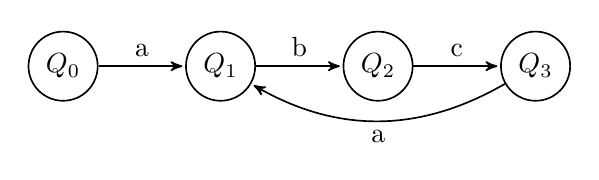
\begin{tikzpicture}[->,>=stealth',shorten >=1pt,auto,node distance=2cm,semithick]
	  \node[state] (A)              {$Q_0$};
	  \node[state] (B) [right of=A] {$Q_1$};
	  \node[state] (C) [right of=B] {$Q_2$};
	  \node[state] (D) [right of=C] {$Q_3$};          
	  \path
(A) edge  node {a} (B)
(B) edge  node {b} (C)
(C) edge  node {c} (D)
(D) edge [bend left]  node {a} (B)
;
	\end{tikzpicture}
  \end{center}
  \end{scriptsize}  
 \caption{\small Four-symbol four-state {\em regular automata} for recognizing the $\{(abc)^n : n \geq 1 \}$ language.}
\label{fig:regautomatae}
\end{figure}

The \strips\ action schema of Figure~\ref{fig:reg-update-rule} models the rule $a,q_0\rightarrow q_1$ of the {\em regular automatae} defined in Figure~\ref{fig:regautomatae}. The full encoding of the {\em automata} of Figure~\ref{fig:regautomatae} produces a total of sixteen \strips\ action schema.

\begin{figure}
\begin{scriptsize}
\begin{lstlisting}
(:action transition-1      ;;; a,$q_0\rightarrow$ $q_1$
  :parameters (?x ?xr)
  :precondition (and (head ?x) (symbol-a ?x) (state-$q_0$)
                     (next ?x ?xr))
  :effect (and (not (head ?x)) 
               (not (symbol-a ?x)) (not (state-$q_0$))
               (head ?xr) (state-$q_1$)))
\end{lstlisting}
\end{scriptsize}
 \caption{\small \strips\ action schema that models the transition $q_0\rightarrow q_1$ of the automata defined in Figure~\ref{fig:regautomatae}.}
\label{fig:regupdate-rule}
\end{figure}



\subsection{Recognition of {\em Turing Machines}}
We analyze now {\em model recognition} when the input set of given set of models represent different {\em Turing machines}.

A {\em Turing machine} is a tuple $\mathcal{M}=\tup{Q,q_o,Q_{\bot},\Sigma,\Upsilon,\square,\delta}$:
\begin{itemize}
\item $Q$ is a finite and non-empty set of machine states with the {\em initial state} $q_0\in Q$ and the {\em terminal states} $Q_{\bot}\subseteq Q$.  
\item $\Sigma$ is the {\em tape alphabet}, a finite non-empty set of symbols with the {\em input alphabet} $\Upsilon\subseteq\Sigma$ (symbols allowed to initially appear in the tape) and the {\em blank symbol} $\square\in\Upsilon$ (the only symbol allowed to occur on the tape infinitely often).
\item $\delta: \Sigma\times (Q\setminus Q_{\bot}) \rightarrow \Sigma\times Q\times\{left,right\}$ is the {\em transition function}. For each pair of tape symbol and non-terminal machine state $\delta$ defines: (1), the tape symbol to print at the current position of the header (2), the new state of the machine and (3), whether the header is shifted {\em left} or {\em right} after the print operation. If $\delta$ is not defined for the current pair of tape symbol and machine state, the machine halts.
\end{itemize}

Figure~\ref{fig:tautomatae} illustrate a seven-symbol six-state {\em Turing Machine} for recognizing the $\{a^nb^nc^n : n \geq 1 \}$ language. The {\em tape alphabet} is $\Sigma=\{a,b,c,x,y,z,\square\}$, the {\em input alphabet} $\Upsilon=\{a,b,c,\square\}$ and the machine states are $Q=\{q_0,q_1,q_2,q_3,q_4,\underline{q_5}\}$ (where \underline{$q_5$} is the only acceptor state).

\begin{figure}
  \begin{scriptsize}
  \begin{center}
	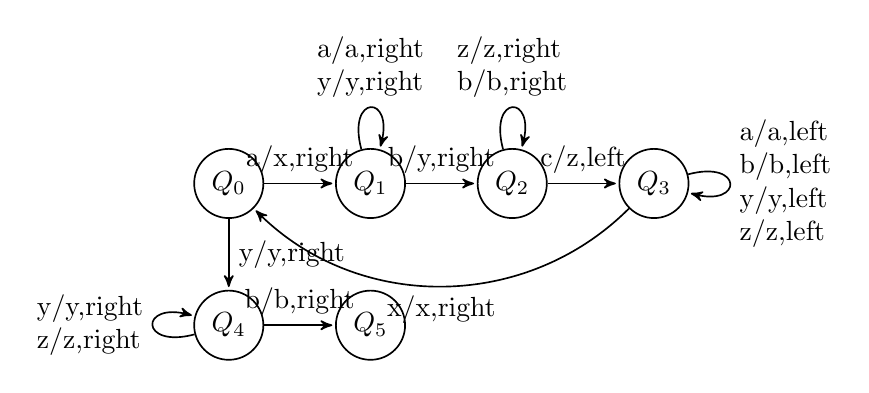
\begin{tikzpicture}[->,>=stealth',shorten >=1pt,auto,node distance=1.8cm,semithick]
	  \node[state] (A)              {$Q_0$};
	  \node[state] (B) [right of=A] {$Q_1$};
	  \node[state] (C) [right of=B] {$Q_2$};
	  \node[state] (D) [right of=C] {$Q_3$};
	  \node[state] (E) [below of=A] {$Q_4$};
	  \node[state] (F) [right of=E] {$Q_5$};                    

	  \path
(A) edge  node {a/x,right} (B)
(B) edge [align=left, loop above] node {a/a,right\\y/y,right} (B)
(B) edge  node {b/y,right} (C)
(C) edge [align=left, loop above] node {z/z,right\\b/b,right} (C)
(C) edge  node {c/z,left} (D)
(D) edge [align=left, loop right] node {a/a,left\\b/b,left\\y/y,left\\z/z,left} (D)
(D) edge [bend left=45] node {x/x,right} (A)

(A) edge  node {y/y,right} (E)
(E) edge [align=left, loop left] node {y/y,right\\z/z,right} (E)
(E) edge  node {b/b,right} (F)
;
	\end{tikzpicture}
  \end{center}
  \end{scriptsize}  
 \caption{\small Seven-symbol six-state {\em Turing Machine} for recognizing the $\{a^nb^nc^n : n \geq 1 \}$ language.}
\label{fig:tautomatae}
\end{figure}


The \strips\ action schema of Figure~\ref{fig:update-rule} models the rule $a,q_0\rightarrow x,r,q_1$ of the {\em Turing Machine} defined in Figure~\ref{fig:tautomatae}. The full encoding of the {\em Turing Machine} of Figure~\ref{fig:tautomatae} produces a total of sixteen \strips\ action schema.

\begin{figure}
\begin{scriptsize}
\begin{lstlisting}
(:action transition-1      ;;; a,$q_0\rightarrow$ x,r,$q_1$
  :parameters (?xl ?x ?xr)
  :precondition (and (head ?x) (symbol-a ?x) (state-$q_0$)
                     (next ?xl ?x) (next ?x ?xr))
  :effect (and (not (head ?x)) 
               (not (symbol-a ?x)) (not (state-$q_0$))
               (head ?xr) (symbol-x ?x) (state-$q_1$)))
\end{lstlisting}
\end{scriptsize}
 \caption{\small \strips\ action schema that models the transition $a,q_0\rightarrow x,r,q_1$ of the Turing Machine defined in Figure~\ref{fig:tautomatae}.}
\label{fig:update-rule}
\end{figure}

With regard to our \strips\ model for {\em Turing Machines}, executions of a {\em Turing Machine} are definable as an action sequence $\tup{a_1, \ldots, a_n}$ that induces the {\em state trajectory} $\tup{s_0, s_1, \ldots, s_n}$ such that $a_i$ ({\small $1\leq i\leq n$}) is applicable in $s_{i-1}$ and generates the successor state $s_i=\theta(s_{i-1},a_i)$. For instance, the execution of the {\em Turing Machine} defined in Figure~\ref{fig:tautomatae} with an initial tape $abc\square\square\square\ldots$ produces the eight-action plan {\small $(a,q_0\rightarrow x,r,q_1)$, $(b,q_1\rightarrow y,r,q_2)$, $(c,q_2\rightarrow z,l,q_3)$, $(y,q_3\rightarrow y,l,q_3)$, $(x,q_3\rightarrow x,r,q_0)$, $(y,q_0\rightarrow y,r,q_4)$, $(z,q_4\rightarrow z,r,q_4)$, $(\square,q_4\rightarrow \square,r,\underline{q_5})$}.

Assuming that the actual applied transitions is unknown means that the observation $\tau$ of the execution of a Turing Machine contains no actions, it is simply a sequence of states $\tau=\tup{s_1, \ldots , s_m}$. Further, assuming that the internal machine state is unknown means that $\tau$ is a $\Phi$-observation and that the $\Phi$ subset does not contain {\small\tt (state-$q$)} fluents, with $q\in Q$ and $q\neq q_0$. Finally, assuming that the values of several tape cells is unknown means that fluents of the kind {\small\tt (symbol-$\sigma$ ?x)} are missing (i.e. unobserved) for some state $s_i\in \tau$ s.t. $1\leq i\leq m$. These facts affects to the a priori probaility of the possible observations.

On the other hand, the model edition for Turing Machines is limited to these subset of possible positive effects: {\tt (head ?xr)} or {\tt (head ?xl)}, {\tt(symbol-$\sigma$ ?x)} with $\sigma \in \Sigma$ and last but not least, {\tt (state-q)} with $q\in Q$. No other positive effects, preconditions, or negative effects are required to be edited. This fact reduces the possible edition operations and affects to the a priori probaility of the possible action models.

\subsection{Results}

\subsection{Conclusions}
\label{sec:conclussions}
The task of {\em model recognition} can also be understood as a classification task where each class is represented with a different planning model and the observed plan execution is the example to classify. With this regard, planning model that is associated to a class is acting as a class prototype that the summarizes all the plan executions that could be synthesized with that model or in other words, all the examples that belong to that class.

In this work we do not assume that the observed agent is acting rationally, like in {\em plan recognition as planning}~\cite{ramirez2012plan,ramirez2009plan}. A related approach is recently followed for {\em model reconciliation}~\cite{Kambhampati:mreconciliation:ijcai17} where model edition is used to conform the PDDL models of two different agents. 

\bibliographystyle{aaai}
\bibliography{planlearnbibliography}

\end{document}
